The general equation of a second degree (In algebraic form) can be expressed as,
\begin{align}
ax^2 + 2bxy + cy^2 + 2dx + 2ey + f = 0 \label{eq:solutions/41/17/eq:2}
\end{align}
The general equation of a second degree (In vector form) can be expressed as,
\begin{align}
\vec{x^T}\vec{V}\vec{x} + 2\vec{u^T}\vec{x} + f = 0
\end{align}
Comparing \eqref{eq:solutions/41/17/eq:1} with \eqref{eq:solutions/41/17/eq:2} , we get,
\begin{align}
a = 2, \ b = -1, \ c = 1, \ d = 1, \ e = -1 \ and \ f = 0
\end{align}
where,
\begin{align}
\vec{V} = \myvec{a & b \\ b & c} = \myvec{2 & -1 \\ -1 & 1} = \vec{V^T}\\
\implies \vec{V} = \myvec{2 & -1 \\ -1 & 1}
\end{align}
and
\begin{align}
\vec{u} = \myvec{1 \\ -1}    
\end{align}
Finding the determinant of V we obtain, 
\begin{align}
|\vec{V}| = 1 > 0
\end{align}
which means the given central conic is an ellipse which can be proven more effectively using,
\begin{align}
\vec{V} = \vec{PDP^T}\label{eq:solutions/41/17/eq:9}    
\end{align}
where $\vec{P}$ is a matrix of Eigen vectors and $\vec{D}$ is a diagonal matrix of Eigen values which will be computed subsequently.\\
Computing Eigen values for $\vec{V}$ using the characteristic equation of the matrix, we get the following quadratic equation in terms of $\lambda$
\begin{align}
\lambda^{2} - 3\lambda + 1 = 0\\
\implies \lambda_{1} = \frac{3 + \sqrt{5}}{2} \ and \ \lambda_{2} = \frac{3 - \sqrt{5}}{2}
\end{align}
Eigen vectors can be computed using the following equation,
\begin{align}
(\lambda\vec{I - V})\vec{p} = 0
\end{align}
Solving this for $\lambda_{1}$ and $\lambda_{2}$ respectively and normalizing them we obtain,
\begin{align}
\vec{p_1} = \sqrt{\frac{2}{5-\sqrt{5}}}\myvec{1 \\[1em] \frac{1-\sqrt{5}}{2}}\\
\vec{p_2} = \sqrt{\frac{2}{5+\sqrt{5}}}\myvec{1 \\[1em] \frac{\sqrt{5}+1}{2}}
\end{align}
Simplifying, 
\begin{align}
\implies \vec{P} = \myvec{\sqrt{\frac{2}{5-\sqrt{5}}} & \sqrt{\frac{2}{5+\sqrt{5}}} \\[1em] \frac{1-\sqrt{5}}{\sqrt{5\sqrt{2}-\sqrt{10}}} & \frac{1+\sqrt{5}}{\sqrt{5\sqrt{2}+\sqrt{10}}}} \label{eq:solutions/41/17/eq:15}
\end{align}
\begin{align}
\vec{D} = \myvec{\frac{3+\sqrt{5}}{2} & 0 \\ 0 & \frac{3-\sqrt{5}}{2}}
\end{align}
Using \eqref{eq:solutions/41/17/eq:9} can verify that it holds which means that the given central conic is an ellipse.
The center of the ellipse can be computed using,
\begin{align}
\vec{c} = \vec{-V^{-1}u}\\
\implies \vec{c} = \myvec{0 \\ 1} \label{eq:solutions/41/17/eq:18}
\end{align}
The parameters of the ellipse are computed as follows,
\begin{align}
\sqrt{\frac{{\vec{u^{T}V^{-1}u} - f}}{\lambda_{1}}} = \sqrt{\frac{3-\sqrt{5}}{2}}\\
\sqrt{\frac{{\vec{u^{T}V^{-1}u} - f}}{\lambda_{2}}} = \sqrt{\frac{3+\sqrt{5}}{2}}
\end{align}
The angle of Rotation can be obtained by equating $\vec{P}$ with the Rotation matrix which is,
\begin{align}
\vec{P} = \myvec{\cos{\theta} & \sin{\theta} \\ -\sin{\theta} & cos{\theta}} \label{eq:solutions/41/17/eq:21}
\end{align}
Comparing \eqref{eq:solutions/41/17/eq:15} and \eqref{eq:solutions/41/17/eq:21} we get,
\begin{align}
\theta = \frac{\pi}{5.66} \label{eq:solutions/41/17/eq:22}  
\end{align}
Using the Affine transformation we find out the actual ellipse,
\begin{align}
\vec{y} = \vec{P^Tx} + \vec{c}     
\end{align}
which means the actual ellipse is obtained by translating and rotating the standard ellipse w.r.t center, $\vec{c}$ from \eqref{eq:solutions/41/17/eq:18} and angle of rotation, $\theta$ from \eqref{eq:solutions/41/17/eq:22} respectively.\\
Using the above data along with $\vec{o}$ (Origin), the center of the standard ellipse, the actual ellipse is plotted as follows.  
\begin{figure}[!ht]
    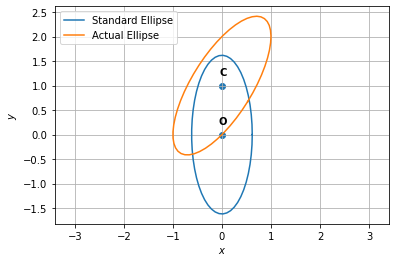
\includegraphics[width=\columnwidth]{solutions/41/17/Figure.png}
    \caption{Standard and Actual Ellipses}
    \label{eq:solutions/41/17/Fig.1}
\end{figure}
